%!TEX program = xelatex
\documentclass[cnfont=NotoCJK]{../simplenote}
\title{SimpleNote笔记模板 v1.1}
\author{Fenglielie \thanks{fenglielie@qq.com}}
\date{\zhtoday}

\usepackage[style=numeric]{biblatex}
\addbibresource{reference.bib} % reference.bib

\usepackage{hologo}

% 主题色的配套颜色定义
\definecolor{ecyan}{RGB}{0,175,152}
\definecolor{eblue}{RGB}{20,50,104}
\definecolor{eblack}{RGB}{0,0,0}


\lstdefinestyle{estyle}{
    basicstyle=%
    \ttfamily
    \lst@ifdisplaystyle\small\fi}

\lstset{language=[LaTeX]TeX,
    style=estyle,
    autogobble=true,
    texcsstyle=*\color[rgb]{0.5,0,0},
    numbers=none,
    breaklines=true,
    keywordstyle=\color[rgb]{0.5,0,0},
    commentstyle=\color{gray},
    emph={%
            fontenc,
            fontspec,
            xeCJK,
            FiraMono,
            xunicode,
            newtxmath,
            figure,
            fig,
            image,
            img,
            table,
            itemize,
            enumerate,
            newtxtext,
            newtxtt,
            ctex,
            microtype,
            description,
            times,
            newtx,
            booktabs,
            tabular,
            PDFLaTeX,
            XeLaTeX,
            type1cm,
            BibTeX,
            device,
            color,
            bg,
            scheme,
            heading,
            fontsize,
            cnfont,
            cite,
            bibstyle,
            math,
            lang,
            amsthm},
    emphstyle={\color[RGB]{190,20,83}},
    morekeywords={%
            DeclareSymbolFont,
            setCJKfamilyfont,
            SetSymbolFont,
            toprule,
            midrule,
            bottomrule,
            includegraphics,
            setmainfont,
            setsansfont,
            setmonofont ,
            setCJKmainfont,
            setCJKsansfont,
            setCJKmonofont,
            RequirePackage,
            figref,eqref,tabref,
            pagecolor,
            definecolor,
            email,
            maketitle,
            keywords,
            printbibliography,addbibresource,parencite
            },
    frame=none,
    tabsize=2}

\begin{document}

\maketitle

SimpleNote是基于\href{https://github.com/ElegantLaTeX/ElegantNote}{ElegantNote}修改的笔记模板,
ElegantNote是非常优秀的一个开源笔记模板,但是原作者在2023年1月1日已经停止更新,因此选择以它的最终版为基础进行魔改,
主要是配置的整理和简化,删除了部分花哨不太实用的配置。


\section{配置说明}

SimpleNote支持两种编译方式:\hologo{pdfLaTeX} 和 \hologo{XeLaTeX}。
支持中文和英文两种模式:英文模式下用任意编译方式均可,中文模式下必须使用 \hologo{XeLaTeX}。
在使用SimpleNote文档类时,有如下主要选项:

\begin{enumerate}
    \item 语言:中文cn(默认),英文en;
    \item 设备:决定页面尺寸,包括 normal(默认,A4)和pad(3:4竖屏);
    \item 颜色:决定主题色,包括\textcolor{eblue}{blue}(默认)、\textcolor{ecyan}{cyan}、 和\textcolor{eblack}{black};
    \item 字号:支持10pt, 11pt(默认), 12pt;
    \item 中文字体:决定中文字体,包括ctex的几个默认方案,以及开源的方正字体,思源字体方案,见下文。
\end{enumerate}



\begin{remark}
    文档类的选项既可以使用完整的键值对形式,例如\lstinline{device=normal},
    也可以直接使用选项名\lstinline{normal},并且多个选项可以连续设置,并且任意顺序均可。
\end{remark}

\subsection{语言}

本模板内含中英文两套语言环境,改变语言会改变图表标题的引导词(图,表),文章结构词(比如目录,参考文献等),以及定理环境中的引导词(比如定理,引理等)。不同语言模式的启用如下:
\begin{lstlisting}[frame=single]
  \documentclass[lang=cn]{simplenote}
  \documentclass[lang=en]{simplenote}
\end{lstlisting}


\begin{note}
    只有中文模式才可输入中文,并且中文要求使用\hologo{XeLaTeX}编译。
    如果需要在英文标准文档类article输入中文,可以将 \lstinline{ctex} 作为宏包导入\footnote{此时更建议直接使用ctexart等中文文档类。}。
    查询\lstinline{ctex}宏包文档可知,默认选项\lstinline{scheme=plain}只提供基本的中文支持功能,而不对文章版式进行任何适合中文排版的修改;
    \lstinline{scheme=chinese}则会修改默认字号为五号字,调整行距为1.3。
    默认选项\lstinline{heading=false},如果设置为\lstinline{heading=true}则会将章节标题和引导词等改为中文。
    如果在标准文档类article中导入ctex宏包并加上上述选项,则与ctexart等中文文档的行为基本一致。
\end{note}


\subsection{纸张}

模板默认背景色为白色,ElegantNote支持为文档类添加选项来自定义护眼背景色,但是我将选项移除了,在导言区仍然可以使用下面语句来配置页面底色:

\begin{lstlisting}[frame=single]
\definecolor{bgcolor}{RGB}{199,237,204}   % 绿豆沙色
\pagecolor{bgcolor}

\definecolor{bgcolor}{RGB}{250,250,248}   % 白底色偏灰
\pagecolor{bgcolor}

\definecolor{bgcolor}{RGB}{250,237,225}   % 秋叶褐色
\pagecolor{bgcolor}
\end{lstlisting}



\subsection{设备}

模板默认尺寸为A4,ElegantNote支持为文档类添加选项来适配不同的设备,这里我仅仅保留了pad的选项,因为随意切换尺寸会非常影响图表的排版效果,也没有太多的必要性。

\begin{lstlisting}[frame=single]
    \documentclass[device=normal]{simplenote}     % A4 page (default)
    \documentclass[device=pad]{simplenote}        % pad 3:4 size
\end{lstlisting}


\subsection[颜色]{颜色\footnote{测试章节的footnote脚注。}}

模板支持不同的颜色主题,分别是 \textcolor{eblue}{blue}(默认),
\textcolor{ecyan}{cyan}和\textcolor{eblack}{black}。
如果不需要颜色,可以选择黑色(black)主题。颜色主题的设置方法:

\begin{lstlisting}[frame=single]
    \documentclass[color=blue]{simplenote} % default
    \documentclass[color=cyan]{simplenote}
    \documentclass[color=black]{simplenote}
\end{lstlisting}

\subsection{字号}

模板支持基本的字号设置,可以选择的值为10pt,11pt(默认),12pt,这和ctex宏包略有不同,用法如下:
\begin{lstlisting}[frame=single]
    \documentclass[fontsize=10pt]{simplenote}
    \documentclass[fontsize=11pt]{simplenote} % default
    \documentclass[fontsize=12pt]{simplenote}
\end{lstlisting}


\subsection{中文字体}

模板支持不同的中文字体配置,通过\lstinline{cnfont=XXX}设置,默认值为\lstinline{cnfont=auto},支持如下的值:
\begin{enumerate}
    \item 兼容ctex宏包关于中文字体的部分选项:
          \begin{enumerate}
              \item \lstinline{cnfont=auto},令ctex根据系统自动选择字体方案
              \item \lstinline{cnfont=windows},令ctex选择windows字体方案(Windows默认)(传递\lstinline{fontset=windows}参数)
              \item \lstinline{cnfont=fandol},令ctex选择fandol字体方案(Linux默认)(传递\lstinline{fontset=fandol}参数)
              \item \lstinline{cnfont=none},禁止ctex的字体配置(传递\lstinline{fontset=none}参数)
          \end{enumerate}
    \item 开源中文字体选项:(向ctex传递\lstinline{fontset=none}参数并自行配置)
          \begin{enumerate}
              \item \lstinline{cnfont=FZ},方正字体(仅使用四个开源字体)
                    \begin{enumerate}
                        \item 方正书宋 FZSSK.TTF,FZShuSong-Z01
                        \item 方正黑体 FZHTK.TTF,FZHei-B01
                        \item 方正楷体 FZKTK.TTF,FZKai-Z03
                        \item 方正仿宋 FZFSK.TTF,FZFangSong-Z02
                    \end{enumerate}
              \item \lstinline{cnfont=NotoCJK},Noto CJK 思源字体(SC简体中文版本)
                    \begin{enumerate}
                        \item 思源宋体 Noto Serif CJK SC
                        \item 思源黑体 Noto Sans CJK SC
                        \item 思源等宽字体 Noto Sans Mono CJK SC
                    \end{enumerate}
              \item \lstinline{cnfont=SourceHan},Source Han 思源字体(SC简体中文版本)
                    \begin{enumerate}
                        \item 思源宋体 Source Han Serif SC
                        \item 思源黑体 Source Han Sans SC
                    \end{enumerate}
          \end{enumerate}
\end{enumerate}

\begin{remark}
    由于思源字体只有思源宋体和思源黑体,缺少通常的楷体(作为宋体的斜体)和仿宋,因此需要使用方正楷体和方正仿宋作为补充,
    换言之,这几个方案都需要安装四个方正开源字体。
\end{remark}

\begin{remark}
    各个在线编译平台(例如Overleaf)支持的中文字体并不统一:
    由于部署在Linux服务器上,fandol字体是最可能可用的,思源字体和windows的字体有时也可用,通常都不含方正开源字体。
\end{remark}

如果选择\lstinline{cnfont=none},还可以自行进行配置,参考代码如下:
\begin{lstlisting}[frame=single]
    \setCJKmainfont{FZShuSong-Z01}[BoldFont={FZHei-B01},ItalicFont={FZKai-Z03}]
    \setCJKsansfont{FZKai-Z03}[BoldFont={FZHei-B01}]
    \setCJKmonofont{FZFangSong-Z02}[BoldFont={FZHei-B01}]

    \setCJKfamilyfont{zhsong}{FZShuSong-Z01}
    \setCJKfamilyfont{zhhei}{FZHei-B01}
    \setCJKfamilyfont{zhkai}{FZKai-Z03}[BoldFont={FZHei-B01}]
    \setCJKfamilyfont{zhfs}{FZFangSong-Z02}[BoldFont={FZHei-B01}]

    \newcommand*{\songti}{\CJKfamily{zhsong}}
    \newcommand*{\heiti}{\CJKfamily{zhhei}}
    \newcommand*{\kaishu}{\CJKfamily{zhkai}}
    \newcommand*{\fangsong}{\CJKfamily{zhfs}}
\end{lstlisting}


\section{使用教程}

\subsection{导言区信息}

在使用模板时的导言区需要如下信息
\begin{lstlisting}[frame=single]
    %!TEX program = xelatex
    \documentclass[cn,blue,14pt,screen]{simplenote}
    \title{标题}
    \author{作者}
    \date{\zhdate{2024/01/13}}% \date{\zhtoday}


    \begin{document}
    ...
    \end{document}
\end{lstlisting}
其中作者可以附带联系方式(使用\lstinline|\thanks{}|命令),可以有多个作者(使用\lstinline|\and|连接),例如
\begin{lstlisting}
    \author{作者一 \thanks{xxxx@xx.xx} \and 作者二}
\end{lstlisting}
中文日期显示命令基于\lstinline{zhnumber}宏包,如果不需要显示日期,不可以省略(默认会自动显示当前英文日期,相当于\lstinline|\date{\today}|),应该留空\lstinline|\date{}|。



\subsection{定理类环境}

本模板支持常见的数学定理环境

\begin{itemize}
    \item \textit{定理类环境},包含标题和内容两部分,全部定理类环境使用全局计数器,计数器相互独立。根据样式的不同可以分为 2 种
          \begin{itemize}
              \item \textbf{definition(定义)} 环境;
              \item \textbf{theorem(定理)、lemma(引理)、corollary(推论)、proposition(命题)} 环境;
          \end{itemize}
    \item \textit{示例与题目},有 \textbf{example(例)、problem(题目)、exercise(练习)}环境,使用各自的全局计数器。
    \item \textit{解答与笔记},有 \textbf{note(笔记)、remark(注)、solution(解)} 环境,无编号。
\end{itemize}
其中定理类环境均有带星号的版本:\textbf{definition*}、\textbf{theorem*}、\textbf{lemma*}、\textbf{corollary*}、\textbf{proposition*},带星号的定理类环境不会编号。
除此之外,还有默认可以使用的\textbf{proof(证明)}环境。


\subsection{交叉引用}

关于交叉引用的命令:ams宏包默认提供了\lstinline|\eqref{}|作为公式的引用命令,但这仅仅是给编号加了括号;
除此之外,本模板还提供了图片的引用命令\lstinline|\figref{}|和表格的引用命令\lstinline|\tabref{}|,实现代码如下,使用效果见下文。
\begin{lstlisting}[frame=single]
    \newcommand\figref[1]{Figure~\ref{#1}}
    \newcommand\tabref[1]{Table~\ref{#1}}
\end{lstlisting}

\subsection{算法环境}

本模板采用algorithm2e宏包来支持算法显示,使用如下,效果如算法~\ref{algorithm:1}。

\begin{lstlisting}[frame=single]
    \begin{algorithm}[H]\label{algorithm:1}
        \caption{Euclid's algorithm}
        \KwData{Two nonnegative integers $a$ and $b$}
        \KwResult{Their greatest common divisor $d = \gcd(a, b)$}
        \While{$b \neq 0$}{
            $r \leftarrow a \bmod b$\;
            $a \leftarrow b$\;
            $b \leftarrow r$\;
        }
        $d \leftarrow a$\;
    \end{algorithm}
\end{lstlisting}


\begin{algorithm}[H]\label{algorithm:1}
    \caption{Euclid's algorithm}
    \KwData{Two nonnegative integers $a$ and $b$}
    \KwResult{Their greatest common divisor $d = \gcd(a, b)$}
    \While{$b \neq 0$}{
        $r \leftarrow a \bmod b$\;
        $a \leftarrow b$\;
        $b \leftarrow r$\;
    }
    $d \leftarrow a$\;
\end{algorithm}

\subsection{代码环境}

本模板采用listings宏包来支持代码高亮显示,使用例如

\begin{lstlisting}[style=simplestyle,language=c++]
#include <iostream>

int main() {
    std::cout << "Hello, world!" << std::endl;
    return 0;
}
\end{lstlisting}

\begin{lstlisting}[style=simplestyle,language=python]
def greet(name):
    """
    greets the person passed in as a parameter.
    """
    print(f"Hello, {name}!")

greet("John")
\end{lstlisting}

\subsection{参考文献}

原本的ElegantNote模板包括了参考文献的部分:使用Biblatex宏包,并支持通过参数传递样式。
但是出于个人需求的原因,将这部分完全移除,在需要参考文献时自行进行配置。

传统的Bibtex的基本用法如下:
\begin{enumerate}
    \item 导言区指定样式,例如\lstinline|\bibliographystyle{plain}|;
    \item 在显示参考文献列表的位置使用\lstinline|\bibliography{reference}|,这里假设参考文献文件为reference.bib。
\end{enumerate}
示例如下:
\begin{lstlisting}[frame=single]
\documentclass{article}
\bibliographystyle{plain}

\begin{document}

According to Einstein's theory of relativity \cite{einstein1905}...

\bibliography{reference} % reference.bib

\end{document}
\end{lstlisting}

现代的Biblatex的基本用法如下:
\begin{enumerate}
    \item 在导言区导入 biblatex 宏包,可以指定样式和后端等;
    \item 在导言区加载参考文献文件,例如\lstinline|\addbibresource[location=local]{reference.bib}|,这里假设参考文献文件为reference.bib
    \item 在显示参考文献列表的位置使用\lstinline|\printbibliography|
\end{enumerate}
示例如下:
\begin{lstlisting}[frame=single]
\documentclass{article}
\usepackage[style=authoryear]{biblatex}
\addbibresource{reference.bib} % reference.bib

\begin{document}

According to Einstein's theory of relativity \parencite{einstein1905}...

\printbibliography[title={References}]

\end{document}
\end{lstlisting}

\section{写作示例}

\begin{theorem}[Fubini 定理]\label{thm:fubi}
    若 $f(x,y)$ 是 $\mathcal{R}^p\times\mathcal{R}^q$ 上的非负可测函数,
    则对几乎处处的 $x\in \mathcal{R}^p$,$f(x,y)$ 作为 $y$ 的函数是 $\mathcal{R}^q$ 上的非负可测函数,
    $g(x)=\int_{\mathcal{R}^q}f(x,y) dy$ 是 $\mathcal{R}^p$ 上的非负可测函数。并且
    \begin{equation}\label{eq:461}
        \int_{\mathcal{R}^p\times\mathcal{R}^q} f(x,y) dxdy=\int_{\mathcal{R}^p}\left(\int_{\mathcal{R}^q}f(x,y)dy\right)dx.
    \end{equation}
\end{theorem}


\begin{theorem}
    对于Burgers方程,假设给定光滑的初值$u_0(x)$,并且存在某些点满足$u_0'(x) < 0$,
    那么准确解在$T_b$时刻特征线首次相交,解出现无穷斜率(间断,激波)。
    \[
        T_b = \frac{-1}{\min u_0'(x)}
    \]
\end{theorem}
\begin{proof}
    证明分成两部分:首先证明在$T_b$时刻特征线首次相交,然后证明在$T_b$时刻会出现无穷斜率,证明细节略。
\end{proof}


\begin{lemma}[Harten引理]
    若差分格式可以表述为如下形式
    \[
        v_j^{n+1} = v_j^n - C_{j-1/2}(v_j^n - v_{j-1}^n) + D_{j+1/2}(v_{j+1}^n - v_j^n)
    \]
    且处处成立
    \[
        C_{j+1/2} \ge 0, D_{j+1/2} \ge 0, C_{j+1/2} + D_{j+1/2} \le 1, \forall j
    \]
    则它是TVD格式。
\end{lemma}

\begin{proposition}
    下面两个结论等价:
    \begin{enumerate}
        \item 存在常数$\delta >0$,使得$A$的所有特征值$\lambda$都满足$\Re\, \lambda \ge \delta$;(即抛物的定义)
        \item 存在常数$\delta >0$,使得$A + A^* \ge \delta I$。
    \end{enumerate}
\end{proposition}

\begin{corollary}
    单调格式一定是TVD格式,TVD格式一定是单调保持格式,反之不成立。
    限于线性差分格式的范畴,单调格式、TVD格式和单调保持格式这三个概念是彼此等价的。
\end{corollary}

\begin{definition}[守恒型格式]
    称差分格式为守恒型格式,若它可以表述为如下形式
    \begin{equation}
        v_{j}^{n+1} = v_j^n - \frac{\Delta t}{\Delta x}\left(
        \hat{f}_{j+1/2}^n - \hat{f}_{j-1/2}^n
        \right) \tag{$*$}
    \end{equation}
    其中$\hat{f}_{j+\frac12}$称为数值流通量,具有表达式$\hat{f}_{j+\frac12} = \hat{f}(v_{j-r},\cdots,v_{j+s})$,
    并且满足
    \begin{enumerate}
        \item 连续性:$\hat{f}$关于每一个变量都是局部Lipschitz连续的
        \item 相容性:$\hat{f}(v,\dots,v) = f(v)$
    \end{enumerate}
\end{definition}


\begin{example}
    Burgers方程$u_t + u u_x = 0$的特征线满足
    \begin{equation}
        \frac{d x}{d t} = f'(u_0(x_0)) = u_0(x_0)
    \end{equation}
    特征线为$x\!-\!t$平面的直线
    \begin{equation}
        x = x_0 + u_0(x_0) t \label{eq:1}
    \end{equation}
\end{example}

下面是图片和表格的示例,其中\figref{fig:1}呈现了一个典型的Burgers方程精确解,
通过求解非线性方程\eqref{eq:1}得到;\tabref{tab:1}呈现了一组数值算法的对比,包括误差和阶数。


\begin{figure}[htbp]
    \centering
    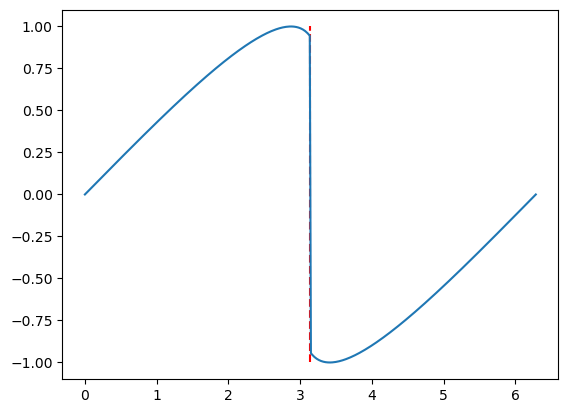
\includegraphics[width=.6\textwidth]{burgers.png}
    \caption{Solution of Burgers' equation}
    \label{fig:1}
\end{figure}

\begin{table}[ht]
    \centering
    \caption{计算结果}\label{tab:1}
    \begin{tabular}{c|c|ccccc}
        \hline
                              &      & N=25     & N=50       & N=100      & N=200      & N=400      \\
        \hline
        \multirow{4}{*}{FTCS} & 误差   & 2.8e-03  & 7.1121e-04 & 1.7821e-04 & 4.4559e-05 & 1.1139e-05 \\
                              & 误差阶数 & -        & 1.97       & 1.99       & 2.00       & 2.00       \\
                              & 时间/s & 0.009449 & 0.009827   & 0.087355   & 0.840438   & 33.303874  \\
        \hline
        \multirow{4}{*}{SVD}  & 误差   & 2.8e-03  & 7.1121e-04 & 1.7847e-04 & 4.4615e-05 & 1.1153e-05 \\
                              & 误差阶数 & -        & 1.97       & 1.99       & 2.00       & 2.00       \\
                              & 时间/s & 0.016365 & 0.010492   & 0.034441   & 0.205993   & 1.431576   \\
        \hline
    \end{tabular}
\end{table}

\begin{problem}
Determine the order of accuracy of the following difference
equations to the partial differential equation
\begin{equation*}
    u_t+au_x=0
\end{equation*}
\begin{equation*}
    v^{n+1}_k=v^{n-1}_k-R\delta_0u^n_k+\frac{R}{6}\delta^2\delta_0u^n_k
\end{equation*}
\end{problem}
\begin{solution}
    截断误差为
    \begin{equation*}
        \begin{aligned}
            T^n_k= & \frac{u^{n+1}_k-u^{n-1}_k}{2\Delta t}+\frac{a}{2\Delta x}(u^n_{k+1}-u^n_{k-1})-\frac{a}{12\Delta x}(u^n_{k+2}-2u^n_{k+1}+2u^n_{k-1}-u^n_{k-2}) \\
            =      & (u_t+\frac{\Delta t^2}{6}u_{ttt}+O(\Delta t^4))|^n_k+a(u_x+\frac{\Delta x^2}{6}u_{xxx}+\frac{\Delta x^4}{120}u_{xxxxx}+O(\Delta x^6))|^n_k     \\
                   & -\frac{a}{12}(2\Delta x^2u_{xxx}+\frac{\Delta x^4}{2}u_{xxxxx}+O(\Delta x^6))|^n_k                                                             \\
            =      & O(\Delta t^2+\Delta x^4)
        \end{aligned}
    \end{equation*}
    关于时间2阶,空间4阶。
\end{solution}

\begin{remark}
    这是remark内容测试。\footfullcite{lubichProjectorsplittingIntegratorDynamical2014}
\end{remark}


\begin{note}
    这是note内容测试。\autocite{kochDynamicalLowRank2007}
\end{note}


多层无序列表效果如下
\begin{itemize}
    \item xxx
    \item xxx
          \begin{itemize}
              \item yyy
              \item yyy
                    \begin{itemize}
                        \item zzz
                        \item zzz
                              \begin{itemize}
                                  \item www
                                  \item www
                              \end{itemize}
                    \end{itemize}
          \end{itemize}
\end{itemize}

多层有序列表效果如下
\begin{enumerate}
    \item xxx
    \item xxx
          \begin{enumerate}
              \item yyy
              \item yyy
                    \begin{enumerate}
                        \item zzz
                        \item zzz
                              \begin{enumerate}
                                  \item www
                                  \item www
                              \end{enumerate}
                    \end{enumerate}
          \end{enumerate}
\end{enumerate}

\nocite{*}
\printbibliography[title={参考文献}]

\end{document}
